\chapter{RBFNN-based identification on an example network}
\label{NN_based_example}

\emph{In Appendix F. a numerical example for the system identification is given. }

\section{The network in EPANET}
\label{example1_EPANET}

The reason for testing the identification method on data from a simple EPANET model is that, in simulation, several different operations of the network can be studied. On a real world network, typically the operation or control cannot be taken to its extremes, as this would mean undesired service to the customers . Therefore, the network shown in \figref{fig:epanet_example1_id} has been created to mimic the behaviour of a multi-inlet, single-WT system, such that the identification method, presented in \chapref{identification_design} is being tested. 

%EPANET example network for identification
\begin{figure}[H]
\centering
%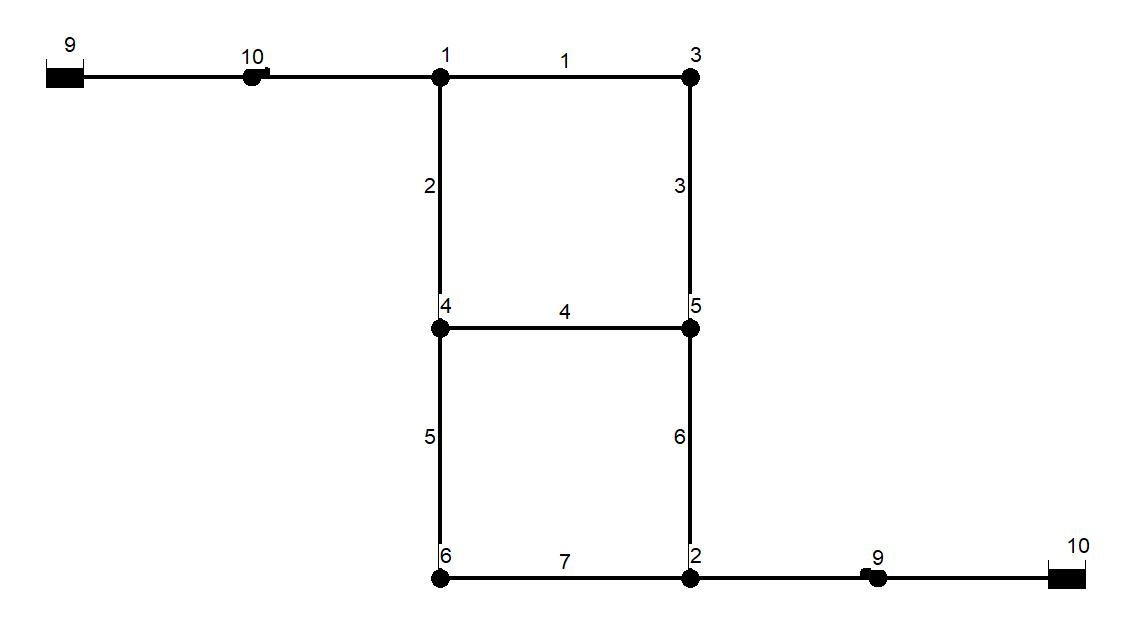
\includegraphics[width=0.6\textwidth]{report/pictures/example1_epanetmodel}
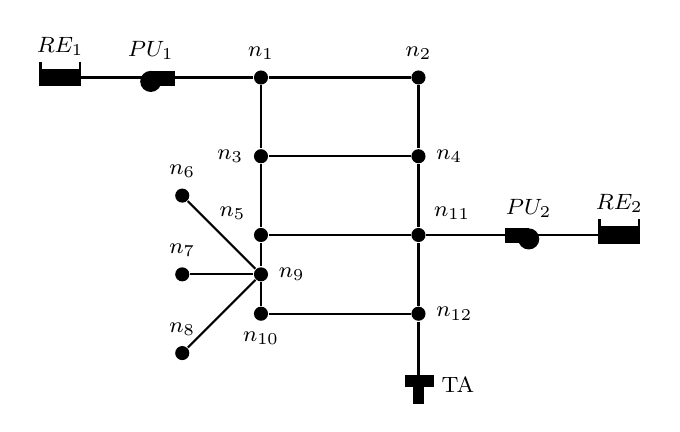
\begin{tikzpicture}[semithick,state/.style ={ draw,shape=circle,scale=0.9}]

\node[circle,fill,inner sep=1.8pt,label=above : \footnotesize$n_1$] (A) at (0,0) {};
\node[circle,fill,inner sep=1.8pt,label=above : \footnotesize$n_2$] (B) at (2,0) {};
\node[circle,fill,inner sep=1.8pt,label= left: \footnotesize$n_3$] (C) at (0,-1) {};
\node[circle,fill,inner sep=1.8pt,label= right: \footnotesize$n_4$] (D) at (2,-1) {};
\node[circle,fill,inner sep=1.8pt,label= above right: \footnotesize $n_{11}$] (E) at (2,-2) {};
\node[circle,fill,inner sep=1.8pt,label= above left: \footnotesize$n_5$] (F) at (0,-2) {};
\node[circle,fill,inner sep=1.8pt,label= below : \footnotesize$n_{10}$] (G) at (0,-3) {};
\node[circle,fill,inner sep=1.8pt,label=  right: \footnotesize$n_9$] (H) at (0,-2.5) {};
\node[circle,fill,inner sep=1.8pt,label=  right: \footnotesize$n_{12}$] (I) at (2,-3) {};
\node[circle,fill,inner sep=1.8pt,label=  above: \footnotesize$n_6$] (J) at (-1,-1.5) {};
\node[circle,fill,inner sep=1.8pt,label=  above: \footnotesize $n_7$] (M) at (-1,-2.5) {};
\node[circle,fill,inner sep=1.8pt,label=  above: \footnotesize $n_8$] (L) at (-1,-3.5) {};



\draw [thick] (A) --  (B) node[above  =0.05 cm] {\footnotesize$$};
\path (A) edge [thick]  node[left  =0.05 cm] {\footnotesize$$} (C);
\path (B) edge [thick] node[right  =0.05 cm] {\footnotesize$$} (D);
\path (C) edge [thick] node[above  =0.05 cm] {\footnotesize$$} (D);
\path (C) edge [thick] node[left  =0.05 cm] {\footnotesize$$} (F);
\path (D) edge [thick] node[right  =0.05 cm] {\footnotesize$$} (E);
\path (E) edge [thick] node[below  =0.05 cm] {\footnotesize$$} (F);
\path (F) edge [thick] node[below  =0.05 cm] {\footnotesize$$} (H);
\path (H) edge [thick] node[below  =0.05 cm] {\footnotesize$$} (G);
\path (H) edge [thick] node[below  =0.05 cm] {\footnotesize$$} (J);
\path (H) edge [thick] node[below  =0.05 cm] {\footnotesize$$} (M);
\path (H) edge [thick] node[below  =0.05 cm] {\footnotesize$$} (L);
\path (G) edge [thick] node[below  =0.05 cm] {\footnotesize$$} (I);
\path (E) edge [thick] node[below  =0.05 cm] {\footnotesize$$} (I);

%PU2
\node[circle,fill,inner sep=2.7pt,label= above : \footnotesize $ PU_2$] (I) at (3.4,-2.05) {};
\draw [thin,fill] (3.1,-1.92) rectangle (3.4,-2.1);


\begin{scope}[xscale=-1,yscale=1]
%PU1
\node[circle,fill,inner sep=2.7pt,label= above : \footnotesize $ PU_1$] (I) at (3.4-2,-2.05+2) {};
\draw [thin,fill] (3.1-2,-1.92+2) rectangle (3.4-2,-2.1+2);

\end{scope}

\draw [thick](2.1,-2) -- (3.1,-2);
\draw [thick, fill] (1.84,-3.79) rectangle (2.18,-3.92);
\draw [thick,fill] (1.95,-3.92) rectangle (2.06,-4.13);
\draw [thick](2,-3.1) -- (2,-3.8);
\node at (2.5,-3.9) {\footnotesize TA};


\draw [thick](-0.1,0) -- (-1.1,0);


\draw [thick](3.5,-2) -- (4.3,-2);
\draw [thick](-1.5,0) -- (-2.3,0);
\draw [thick](-2.3,0.2) -- (-2.3,-0.1) -- (-2.8,-0.1) -- (-2.8,0.2);
\draw [thick,fill] (-2.8,0.1) rectangle (-2.3,-0.1);
\draw [thick](4.3,-1.8) -- (4.3,-2.1) -- (4.8,-2.1) -- (4.8,-1.8);
\draw [thick,fill] (4.3,-1.9) rectangle (4.8,-2.1);
\node at (-2.55,0.4) {\footnotesize $RE_1$};
\node at (4.55,-1.6) {\footnotesize $RE_2$};
\end{tikzpicture} 
\caption{Multi-inlet, Single-WT example network.}
\label{fig:epanet_example1_id}
\end{figure}
\vspace{-3mm}

The network shown in \figref{fig:epanet_example1_id} consists of two pumping stations $PU_1$ and $PU_2$ and a Water Tank $TA$. Furthermore, reservoirs are present in the network, as in EPANET reservoirs are required for simulating pumps. These reservoirs $RE_1$ and $RE_2$ are different from WTs in the sense that they cannot be emptied in the simulation. Additionally, the physical and operational properties of the network can be found in \appref{physical_properties_example1}. 

The controls implemented on the network are based on simple time scheduling of the two pumping stations. Both pumps turn off when the pressure head in the WT is above $19.85 [m]$. $PU_2$ turns on again if the pressure head in the WT decreases to $19.55 [m]$. Furthermore, $PU_2$ turns on again only if the pressure head in node $n_1$ exceeds $43 [m]$. The initial pressure head in the WT is $19.5 [m]$.

\section{Identification and validation}
\label{identification_and_validation_of_the_output_eq} 

The identification is carried out on the simulation data, exported from EPANET. In order to validate the identified model, scenarios with increased and decreased consumption patterns are taken intro account. It is worth noting, that the control properties of the network are kept the same, as any modification in control would mean a new operating point in the WSS. Thus, the model is tested by modifying the total demand and therefore creating different inlet pressure and flow settings for the two pumping stations. The identification is carried out on the network when the total consumption is $\sigma_1$. The validation is done when the total consumption is increased($\sigma_2$) and when decreased($\sigma_3$), respectively. Furthermore, all three consumption curves are periodic with a time period of 24 hours, however the validation has been done on a 72 hours long test data. \figref{fig:sigma123} shows the three different consumption patterns.

  %Total consumptions
 \begin{figure}[H]
 \centering
 %\hspace{0mm}
 %
\includegraphics[width=0.35\textwidth]{report/pictures/missingfigure}
 % This file was created by matlab2tikz.
%
%The latest updates can be retrieved from
%  http://www.mathworks.com/matlabcentral/fileexchange/22022-matlab2tikz-matlab2tikz
%where you can also make suggestions and rate matlab2tikz.
%
\definecolor{mycolor1}{rgb}{0.00000,0.44700,0.74100}%
\definecolor{mycolor2}{rgb}{0.85000,0.32500,0.09800}%
\definecolor{mycolor3}{rgb}{0.92900,0.69400,0.12500}%
%
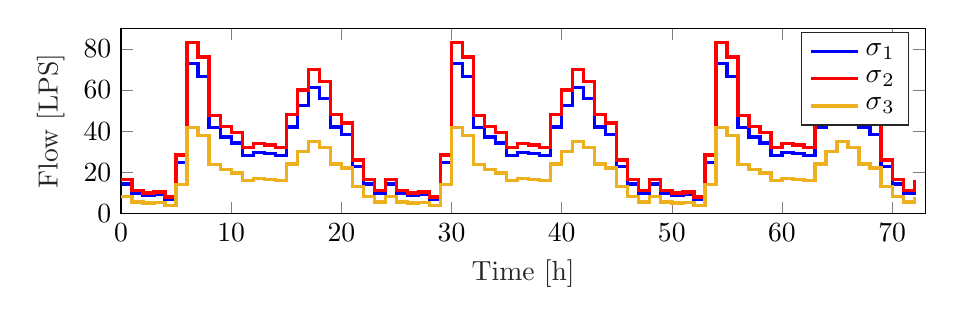
\begin{tikzpicture}

\begin{axis}[%
width=4.021in,
height=0.926in,
at={(0.758in,0.481in)},
scale only axis,
xmin=0,
xmax=73,
xlabel style={font=\color{white!15!black}},
xlabel={Time [h]},
ymin=0,
ymax=90,
ylabel style={font=\color{white!15!black}},
ylabel={Flow  [LPS]},
axis background/.style={fill=white},
legend style={legend cell align=left, align=left, draw=white!15!black}
]
\addplot[const plot, color=blue, line width=1.2pt] table[row sep=crcr] {%
0	14.35\\
1	9.8\\
2	8.75\\
3	9.1\\
4	7\\
5	24.85\\
6	72.8\\
7	66.5\\
8	41.65\\
9	37.1\\
10	34.3\\
11	28\\
12	29.75\\
13	29.05\\
14	28\\
15	42\\
16	52.5\\
17	61.25\\
18	56\\
19	42\\
20	38.5\\
21	22.75\\
22	14.35\\
23	9.8\\
24	14.35\\
25	9.8\\
26	8.75\\
27	9.1\\
28	7\\
29	24.85\\
30	72.8\\
31	66.5\\
32	41.65\\
33	37.1\\
34	34.3\\
35	28\\
36	29.75\\
37	29.05\\
38	28\\
39	42\\
40	52.5\\
41	61.25\\
42	56\\
43	42\\
44	38.5\\
45	22.75\\
46	14.35\\
47	9.8\\
48	14.35\\
49	9.8\\
50	8.75\\
51	9.1\\
52	7\\
53	24.85\\
54	72.8\\
55	66.5\\
56	41.65\\
57	37.1\\
58	34.3\\
59	28\\
60	29.75\\
61	29.05\\
62	28\\
63	42\\
64	52.5\\
65	61.25\\
66	56\\
67	42\\
68	38.5\\
69	22.75\\
70	14.35\\
71	9.8\\
72	14.35\\
};
\addlegendentry{$\sigma{}_\text{1}$}

\addplot[const plot, color=red, line width=1.2pt] table[row sep=crcr] {%
0	16.4\\
1	11.2\\
2	10\\
3	10.4\\
4	8\\
5	28.4\\
6	83.2\\
7	76\\
8	47.6\\
9	42.4\\
10	39.2\\
11	32\\
12	34\\
13	33.2\\
14	32\\
15	48\\
16	60\\
17	70\\
18	64\\
19	48\\
20	44\\
21	26\\
22	16.4\\
23	11.2\\
24	16.4\\
25	11.2\\
26	10\\
27	10.4\\
28	8\\
29	28.4\\
30	83.2\\
31	76\\
32	47.6\\
33	42.4\\
34	39.2\\
35	32\\
36	34\\
37	33.2\\
38	32\\
39	48\\
40	60\\
41	70\\
42	64\\
43	48\\
44	44\\
45	26\\
46	16.4\\
47	11.2\\
48	16.4\\
49	11.2\\
50	10\\
51	10.4\\
52	8\\
53	28.4\\
54	83.2\\
55	76\\
56	47.6\\
57	42.4\\
58	39.2\\
59	32\\
60	34\\
61	33.2\\
62	32\\
63	48\\
64	60\\
65	70\\
66	64\\
67	48\\
68	44\\
69	26\\
70	16.4\\
71	11.2\\
72	16.4\\
};
\addlegendentry{$\sigma{}_\text{2}$}

\addplot[const plot, color=mycolor3, line width=1.2pt] table[row sep=crcr] {%
0	8.2\\
1	5.6\\
2	5\\
3	5.2\\
4	4\\
5	14.2\\
6	41.6\\
7	38\\
8	23.8\\
9	21.2\\
10	19.6\\
11	16\\
12	17\\
13	16.6\\
14	16\\
15	24\\
16	30\\
17	35\\
18	32\\
19	24\\
20	22\\
21	13\\
22	8.2\\
23	5.6\\
24	8.2\\
25	5.6\\
26	5\\
27	5.2\\
28	4\\
29	14.2\\
30	41.6\\
31	38\\
32	23.8\\
33	21.2\\
34	19.6\\
35	16\\
36	17\\
37	16.6\\
38	16\\
39	24\\
40	30\\
41	35\\
42	32\\
43	24\\
44	22\\
45	13\\
46	8.2\\
47	5.6\\
48	8.2\\
49	5.6\\
50	5\\
51	5.2\\
52	4\\
53	14.2\\
54	41.6\\
55	38\\
56	23.8\\
57	21.2\\
58	19.6\\
59	16\\
60	17\\
61	16.6\\
62	16\\
63	24\\
64	30\\
65	35\\
66	32\\
67	24\\
68	22\\
69	13\\
70	8.2\\
71	5.6\\
72	8.2\\
};
\addlegendentry{$\sigma{}_\text{3}$}

\end{axis}
\end{tikzpicture}% 
 \vspace{-2.5mm}
 \caption{Consumption patterns used for identification and validation.}
 \label{fig:sigma123}
 \end{figure}

 \vspace{-3mm}

 The inlet flows of the two pumping stations $PU_1$ and $PU_2$, and the WT pressure $\hat{p}$ are shown in \figref{fig:WT_sigma1}. 

 \vspace{-3mm}

   %Inlet flow - sigma1
 \begin{figure}[H]
 \centering
 %\hspace{0mm}
 %
\includegraphics[width=0.35\textwidth]{report/pictures/missingfigure}
 % This file was created by matlab2tikz.
%
%The latest updates can be retrieved from
%  http://www.mathworks.com/matlabcentral/fileexchange/22022-matlab2tikz-matlab2tikz
%where you can also make suggestions and rate matlab2tikz.
%
\definecolor{mycolor1}{rgb}{0.00000,0.44700,0.74100}%
\definecolor{mycolor2}{rgb}{0.85000,0.32500,0.09800}%
%
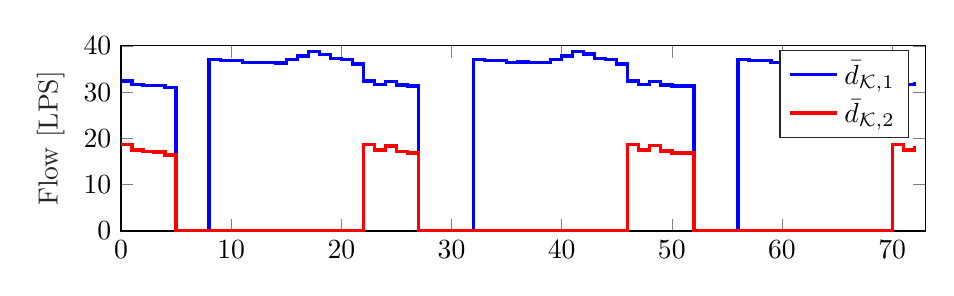
\begin{tikzpicture}

\begin{axis}[%
width=4.021in,
height=0.926in,
at={(0.75in,0.431in)},
scale only axis,
xmin=0,
xmax=73,
%xlabel style={font=\color{white!15!black}},
%xlabel={Time [h]},
ymin=0,
ymax=40,
ylabel style={font=\color{white!15!black}},
ylabel={Flow  [LPS]},
axis background/.style={fill=white},
legend style={legend cell align=left, align=left, draw=white!15!black}
]
\addplot[const plot, color=blue, line width=1.2pt] table[row sep=crcr] {%
0	32.41\\
1	31.67\\
2	31.44\\
3	31.42\\
4	31.03\\
5	0\\
6	0\\
7	0\\
8	37.09\\
9	36.88\\
10	36.76\\
11	36.37\\
12	36.46\\
13	36.4\\
14	36.31\\
15	37.04\\
16	37.78\\
17	38.7\\
18	38.19\\
19	37.19\\
20	37.02\\
21	36.06\\
22	32.4\\
23	31.67\\
24	32.26\\
25	31.53\\
26	31.3\\
27	0\\
28	0\\
29	0\\
30	0\\
31	0\\
32	37.11\\
33	36.9\\
34	36.78\\
35	36.38\\
36	36.48\\
37	36.42\\
38	36.33\\
39	37.05\\
40	37.8\\
41	38.71\\
42	38.21\\
43	37.21\\
44	37.04\\
45	36.07\\
46	32.42\\
47	31.68\\
48	32.27\\
49	31.54\\
50	31.31\\
51	31.29\\
52	0\\
53	0\\
54	0\\
55	0\\
56	37.1\\
57	36.9\\
58	36.77\\
59	36.38\\
60	36.48\\
61	36.41\\
62	36.32\\
63	37.05\\
64	37.8\\
65	38.71\\
66	38.21\\
67	37.2\\
68	37.04\\
69	36.07\\
70	32.42\\
71	31.68\\
72	32.27\\
};
\addlegendentry{$\bar{d}_{\mathcal{K},1}$}

\addplot[const plot, color=red, line width=1.2pt] table[row sep=crcr] {%
0	18.64\\
1	17.5\\
2	17.12\\
3	17.07\\
4	16.43\\
5	0\\
6	0\\
7	0\\
8	0\\
9	0\\
10	0\\
11	0\\
12	0\\
13	0\\
14	0\\
15	0\\
16	0\\
17	0\\
18	0\\
19	0\\
20	0\\
21	0\\
22	18.63\\
23	17.49\\
24	18.39\\
25	17.24\\
26	16.86\\
27	0\\
28	0\\
29	0\\
30	0\\
31	0\\
32	0\\
33	0\\
34	0\\
35	0\\
36	0\\
37	0\\
38	0\\
39	0\\
40	0\\
41	0\\
42	0\\
43	0\\
44	0\\
45	0\\
46	18.65\\
47	17.51\\
48	18.41\\
49	17.26\\
50	16.88\\
51	16.84\\
52	0\\
53	0\\
54	0\\
55	0\\
56	0\\
57	0\\
58	0\\
59	0\\
60	0\\
61	0\\
62	0\\
63	0\\
64	0\\
65	0\\
66	0\\
67	0\\
68	0\\
69	0\\
70	18.65\\
71	17.51\\
72	18.41\\
};
\addlegendentry{ $\bar{d}_{\mathcal{K},2}$}

\end{axis}
\end{tikzpicture}% 
 \vspace{-2.5mm}
 %\caption{Inlet flows of $PU_1$ and $PU_2$.}
 \label{fig:dk_sigma1}
 \end{figure}

 \vspace{-6.5mm}

   %WT - sigma1
 \begin{figure}[H]
 \centering
 \hspace{-4.5mm}
 %
\includegraphics[width=0.35\textwidth]{report/pictures/missingfigure}
 % This file was created by matlab2tikz.
%
%The latest updates can be retrieved from
%  http://www.mathworks.com/matlabcentral/fileexchange/22022-matlab2tikz-matlab2tikz
%where you can also make suggestions and rate matlab2tikz.
%
\definecolor{mycolor1}{rgb}{0.00000,0.44700,0.74100}%
%
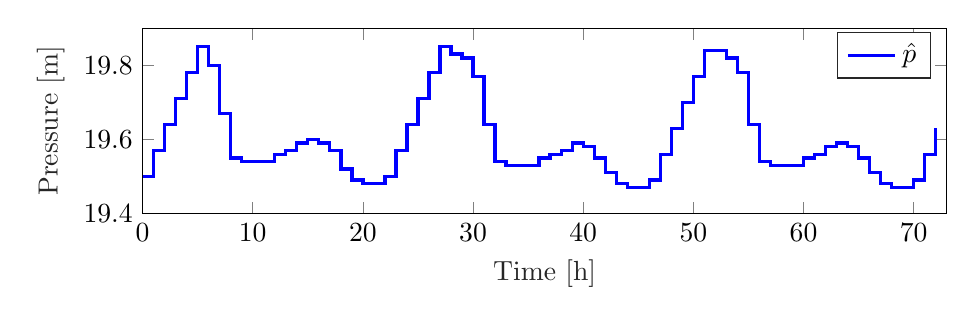
\begin{tikzpicture}

\begin{axis}[%
width=4.021in,
height=0.926in,
at={(0.792in,0.434in)},
scale only axis,
xmin=0,
xmax=73,
xlabel style={font=\color{white!15!black}},
xlabel={Time [h]},
ymin=19.4,
ymax=19.9,
ylabel style={font=\color{white!15!black}},
ylabel={Pressure  [m]},
axis background/.style={fill=white},
legend style={legend cell align=left, align=left, draw=white!15!black}
]
\addplot[const plot, color=blue, line width=1.2pt] table[row sep=crcr] {%
0	19.5\\
1	19.57\\
2	19.64\\
3	19.71\\
4	19.78\\
5	19.85\\
6	19.8\\
7	19.67\\
8	19.55\\
9	19.54\\
10	19.54\\
11	19.54\\
12	19.56\\
13	19.57\\
14	19.59\\
15	19.6\\
16	19.59\\
17	19.57\\
18	19.52\\
19	19.49\\
20	19.48\\
21	19.48\\
22	19.5\\
23	19.57\\
24	19.64\\
25	19.71\\
26	19.78\\
27	19.85\\
28	19.83\\
29	19.82\\
30	19.77\\
31	19.64\\
32	19.54\\
33	19.53\\
34	19.53\\
35	19.53\\
36	19.55\\
37	19.56\\
38	19.57\\
39	19.59\\
40	19.58\\
41	19.55\\
42	19.51\\
43	19.48\\
44	19.47\\
45	19.47\\
46	19.49\\
47	19.56\\
48	19.63\\
49	19.7\\
50	19.77\\
51	19.84\\
52	19.84\\
53	19.82\\
54	19.78\\
55	19.64\\
56	19.54\\
57	19.53\\
58	19.53\\
59	19.53\\
60	19.55\\
61	19.56\\
62	19.58\\
63	19.59\\
64	19.58\\
65	19.55\\
66	19.51\\
67	19.48\\
68	19.47\\
69	19.47\\
70	19.49\\
71	19.56\\
72	19.63\\
};
\addlegendentry{$\hat{p}$}

\end{axis}
\end{tikzpicture}% 
 \vspace{-2.5mm}
 \caption{Inlet flows of $PU_1$ and $PU_2$(above) and the pressure in the WT(below) under $\sigma_1$ total demands.}
 \label{fig:WT_sigma1}
 \end{figure}

 \vspace{-3mm}

 \subsection{Identification on $\sigma_1$ total demands}
 \label{identification_sigma1}

For the two inlet pressures $\bar{p}_{\mathcal{K}1}$ and $\bar{p}_{\mathcal{K}2}$, the identification has been carried out with ten RBF neurons. The performance goal has been chosen to the order of $10^{-4}$. \figref{fig:MSE_output} shows the mean of squared errors in terms of RBF neurons. 

   %MSE output
 \begin{figure}[H]
 \centering
 %\hspace{0mm}
 %
\includegraphics[width=0.35\textwidth]{report/pictures/missingfigure}
 % This file was created by matlab2tikz.
%
%The latest updates can be retrieved from
%  http://www.mathworks.com/matlabcentral/fileexchange/22022-matlab2tikz-matlab2tikz
%where you can also make suggestions and rate matlab2tikz.
%
\definecolor{mycolor1}{rgb}{0.92900,0.69400,0.12500}%
\definecolor{mycolor2}{rgb}{0.49400,0.18400,0.55600}%
%
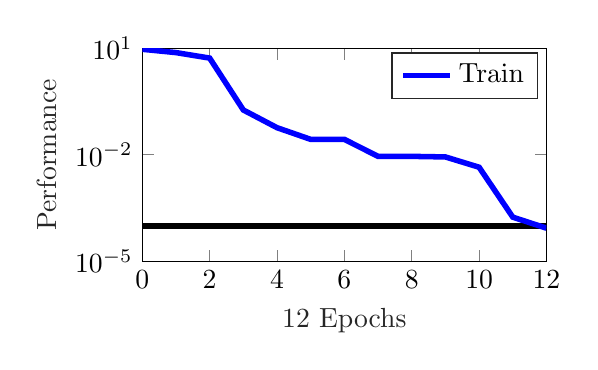
\begin{tikzpicture}

\begin{axis}[%
width=2.021in,
height=1.066in,
at={(0.758in,0.481in)},
scale only axis,
xmin=0,
xmax=12,
xlabel style={font=\color{white!15!black}},
xlabel={12 Epochs},
ymode=log,
ymin=1e-05,
ymax=10,
yminorticks=true,
ylabel style={font=\color{white!15!black}},
ylabel={Performance},
axis background/.style={fill=white},
%title style={font=\bfseries},
%title={Performance is 8.59528e-05, Goal is 0.0001},
legend style={legend cell align=left, align=left, draw=white!15!black}
]
\addplot [color=black, line width=2.0pt, forget plot]
  table[row sep=crcr]{%
0	0.0001\\
1	0.0001\\
2	0.0001\\
3	0.0001\\
4	0.0001\\
5	0.0001\\
6	0.0001\\
7	0.0001\\
8	0.0001\\
9	0.0001\\
10	0.0001\\
11	0.0001\\
12	0.0001\\
};
\addplot [color=blue, line width=2.0pt]
  table[row sep=crcr]{%
0	9.30084312163891\\
1	7.50455220664665\\
2	5.25664645000706\\
3	0.182039469478282\\
4	0.0578400961928023\\
5	0.0271025396912597\\
6	0.0271025396912595\\
7	0.00901207565548084\\
8	0.00901207565548112\\
9	0.00868579632596006\\
10	0.00445311736376068\\
11	0.000175417298503374\\
12	8.59528424540216e-05\\
};
\addlegendentry{Train}

\addplot [color=mycolor1, forget plot]
  table[row sep=crcr]{%
0	0\\
};
\addplot [color=mycolor2, forget plot]
  table[row sep=crcr]{%
0	0\\
};
\end{axis}
\end{tikzpicture}% 
 \vspace{-2.5mm}
 \caption{The network’s performance according to the mean of squared errors.}
 \label{fig:MSE_output}
 \end{figure}

 \vspace{-4mm}

As it is shown in \figref{fig:MSE_output}, a very accurate fit is achieved for the model which is capable of generalizing the output equation. It is worth to mention that although more RBF neurons results in a more accurate fit, however it does not generalize the model as well as ten RBF neurons. In case of increasing the number of neurons, the identification resulted in overfit and the validation failed. The identification of $\bar{p}_{\mathcal{K}1}$ and $\bar{p}_{\mathcal{K}2}$ inlet pressures in case of $\sigma_1$ total demand is shown in \figref{fig:pk1_sigma1}.

\vspace{-2mm}

   %pk1 - pk2 - sigma1
 \begin{figure}[H]
 \centering
 %\hspace{0mm}
 %
\includegraphics[width=0.35\textwidth]{report/pictures/missingfigure}
 % This file was created by matlab2tikz.
%
%The latest updates can be retrieved from
%  http://www.mathworks.com/matlabcentral/fileexchange/22022-matlab2tikz-matlab2tikz
%where you can also make suggestions and rate matlab2tikz.
%
\definecolor{mycolor1}{rgb}{0.00000,0.44700,0.74100}%
\definecolor{mycolor2}{rgb}{0.85000,0.32500,0.09800}%
%
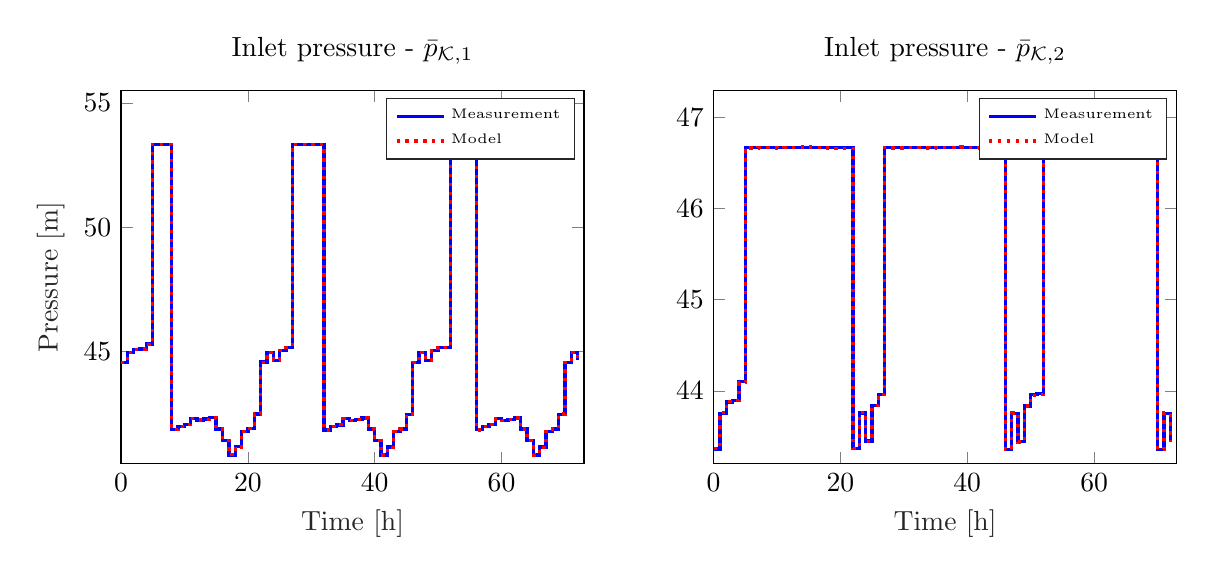
\begin{tikzpicture}

\begin{axis}[%
width=2.315in,
height=1.866in,
at={(0.796in,0.481in)},
scale only axis,
xmin=0,
xmax=73,
xlabel style={font=\color{white!15!black}},
xlabel={Time [h]},
ymin=40.5,
ymax=55.5,
ylabel style={font=\color{white!15!black}},
ylabel={Pressure  [m]},
axis background/.style={fill=white},
%title style={font=\bfseries},
title={Inlet pressure - $\bar{p}_{\mathcal{K},1}$},
legend style={legend cell align=left, align=left, draw=white!15!black}
]
\addplot[const plot, color=blue, line width=1.2pt] table[row sep=crcr] {%
0	44.5758988946\\
1	44.9710905074\\
2	45.0920610176\\
3	45.1025385224\\
4	45.3055172594\\
5	53.33\\
6	53.33\\
7	53.33\\
8	41.8651820546\\
9	41.9946399104\\
10	42.0682858016\\
11	42.3059773154\\
12	42.2513504456\\
13	42.28778336\\
14	42.3423202226\\
15	41.8960720256\\
16	41.4346451144\\
17	40.84825154\\
18	41.1750601826\\
19	41.8032771026\\
20	41.9084163464\\
21	42.4931031176\\
22	44.58130016\\
23	44.9710905074\\
24	44.6567428616\\
25	45.0448297394\\
26	45.16526354\\
27	53.33\\
28	53.33\\
29	53.33\\
30	53.33\\
31	53.33\\
32	41.8528143986\\
33	41.98234226\\
34	42.0560281544\\
35	42.2999143304\\
36	42.2391928064\\
37	42.2756457224\\
38	42.3302125874\\
39	41.889897365\\
40	41.42204744\\
41	40.8418001906\\
42	41.1623258306\\
43	41.7908761106\\
44	41.8960720256\\
45	42.4870918034\\
46	44.5704959624\\
47	44.9658109184\\
48	44.6513649314\\
49	45.0395734856\\
50	45.1600456226\\
51	45.1704797906\\
52	53.33\\
53	53.33\\
54	53.33\\
55	53.33\\
56	41.85899906\\
57	41.98234226\\
58	42.0621578114\\
59	42.2999143304\\
60	42.2391928064\\
61	42.2817153746\\
62	42.3362672384\\
63	41.889897365\\
64	41.42204744\\
65	40.8418001906\\
66	41.1623258306\\
67	41.79707744\\
68	41.8960720256\\
69	42.4870918034\\
70	44.5704959624\\
71	44.9658109184\\
72	44.6513649314\\
};
\addlegendentry{\tiny Measurement}

\addplot[const plot, color=red, dotted, line width=1.2pt] table[row sep=crcr] {%
0	44.5701885077527\\
1	44.9762262146865\\
2	45.095378141338\\
3	45.1031927871572\\
4	45.2941366457955\\
5	53.3275723011397\\
6	53.332462156663\\
7	53.3357109437853\\
8	41.8645363966464\\
9	41.9963483286344\\
10	42.0735721809112\\
11	42.3055764625103\\
12	42.2519443139171\\
13	42.2864577927572\\
14	42.3382694095733\\
15	41.899205563181\\
16	41.4408683011668\\
17	40.854218296608\\
18	41.1696327876139\\
19	41.7977140425853\\
20	41.9055852902994\\
21	42.4932716366776\\
22	44.5760806811398\\
23	44.9770169280414\\
24	44.6628624260891\\
25	45.0469256578999\\
26	45.1611778499202\\
27	53.3344702372491\\
28	53.3302273174497\\
29	53.3298855712179\\
30	53.32600181302\\
31	53.3292584558483\\
32	41.8521631096744\\
33	41.9845731467987\\
34	42.0622039726051\\
35	42.2999806068884\\
36	42.241312478622\\
37	42.2759477139188\\
38	42.3270924746935\\
39	41.8918101059633\\
40	41.4273987292464\\
41	40.8420342383436\\
42	41.155893901885\\
43	41.7852816799597\\
44	41.8936016998919\\
45	42.4884968476104\\
46	44.5646018168106\\
47	44.9717932237981\\
48	44.6564557121393\\
49	45.0418231438692\\
50	45.1564328687633\\
51	45.1640298300379\\
52	53.3272062310905\\
53	53.3298855712179\\
54	53.3281560610623\\
55	53.3292584558483\\
56	41.8571694951758\\
57	41.9845731467987\\
58	42.0670798774855\\
59	42.2999806068884\\
60	42.241312478622\\
61	42.2807095005846\\
62	42.3326816792752\\
63	41.8918101059633\\
64	41.4273987292464\\
65	40.8420342383436\\
66	41.155893901885\\
67	41.79029993703\\
68	41.8936016998919\\
69	42.4884968476104\\
70	44.5646018168106\\
71	44.9717932237981\\
72	44.6564557127222\\
};
\addlegendentry{\tiny Model}

\end{axis}

\begin{axis}[%
xshift=1cm,
width=2.315in,
height=1.866in,
at={(3.365in,0.481in)},
scale only axis,
xmin=0,
xmax=73,
xlabel style={font=\color{white!15!black}},
xlabel={Time [h]},
ymin=43.2,
ymax=47.3,
%ylabel style={font=\color{white!15!black}},
%ylabel={Pressure  [m]},
axis background/.style={fill=white},
%title style={font=\bfseries},
title={Inlet pressure - $\bar{p}_{\mathcal{K},2}$},
legend style={legend cell align=left, align=left, draw=white!15!black}
]
\addplot[const plot, color=blue, line width=1.2pt] table[row sep=crcr] {%
0	43.36054256\\
1	43.75296875\\
2	43.87827584\\
3	43.8945588275\\
4	44.0987748275\\
5	46.67\\
6	46.67\\
7	46.67\\
8	46.67\\
9	46.67\\
10	46.67\\
11	46.67\\
12	46.67\\
13	46.67\\
14	46.67\\
15	46.67\\
16	46.67\\
17	46.67\\
18	46.67\\
19	46.67\\
20	46.67\\
21	46.67\\
22	43.3640925275\\
23	43.7563015475\\
24	43.4487202475\\
25	43.83900236\\
26	43.96242731\\
27	46.67\\
28	46.67\\
29	46.67\\
30	46.67\\
31	46.67\\
32	46.67\\
33	46.67\\
34	46.67\\
35	46.67\\
36	46.67\\
37	46.67\\
38	46.67\\
39	46.67\\
40	46.67\\
41	46.67\\
42	46.67\\
43	46.67\\
44	46.67\\
45	46.67\\
46	43.3569906875\\
47	43.7496340475\\
48	43.4417098475\\
49	43.83243011\\
50	43.95599984\\
51	43.96884716\\
52	46.67\\
53	46.67\\
54	46.67\\
55	46.67\\
56	46.67\\
57	46.67\\
58	46.67\\
59	46.67\\
60	46.67\\
61	46.67\\
62	46.67\\
63	46.67\\
64	46.67\\
65	46.67\\
66	46.67\\
67	46.67\\
68	46.67\\
69	46.67\\
70	43.3569906875\\
71	43.7496340475\\
72	43.4417098475\\
};
\addlegendentry{\tiny Measurement}

\addplot[const plot, color=red, dotted, line width=1.2pt] table[row sep=crcr] {%
0	43.3634086869052\\
1	43.7606129460834\\
2	43.8816726028965\\
3	43.8931366141121\\
4	44.0928387397082\\
5	46.6691685405911\\
6	46.6670879108031\\
7	46.6699851678146\\
8	46.6721652465749\\
9	46.6698102009525\\
10	46.6684039738305\\
11	46.6717347651268\\
12	46.6738844581067\\
13	46.6760095708957\\
14	46.6794689811097\\
15	46.6790770477246\\
16	46.6750852208527\\
17	46.6706281159638\\
18	46.6682393693361\\
19	46.6640028669002\\
20	46.661867590035\\
21	46.6641090317531\\
22	43.3664326699137\\
23	43.7625180157117\\
24	43.4430275595152\\
25	43.8372384385081\\
26	43.957131210854\\
27	46.6742975390751\\
28	46.6690409582936\\
29	46.6687257060116\\
30	46.6701349748723\\
31	46.6723613261931\\
32	46.6703778714421\\
33	46.6678940257557\\
34	46.6664218872324\\
35	46.6703202569629\\
36	46.6718251626263\\
37	46.6739418955784\\
38	46.6766429846536\\
39	46.6779403115681\\
40	46.6736973295969\\
41	46.6703277579328\\
42	46.6669990057898\\
43	46.6622222464899\\
44	46.6599842121484\\
45	46.6626572589573\\
46	43.3593609408211\\
47	43.7567616521063\\
48	43.4369925507439\\
49	43.8315037477686\\
50	43.9514843165921\\
51	43.9612395043769\\
52	46.669117855472\\
53	46.6687257060116\\
54	46.6691192986702\\
55	46.6723613261931\\
56	46.6710170621648\\
57	46.6678940257557\\
58	46.6670819407595\\
59	46.6703202569629\\
60	46.6718251626263\\
61	46.6746078225204\\
62	46.6780561194514\\
63	46.6779403115681\\
64	46.6736973295969\\
65	46.6703277579328\\
66	46.6669990057898\\
67	46.6628625078697\\
68	46.6599842121484\\
69	46.6626572589573\\
70	43.3593609408211\\
71	43.7567616521063\\
72	43.4369925507449\\
};
\addlegendentry{\tiny Model}

\end{axis}
\end{tikzpicture}% 
 \vspace{-2.5mm}
 \caption{Identification of the inlet pressures $\bar{p}_{\mathcal{K}1}$ and $\bar{p}_{\mathcal{K}2}$.}
 \label{fig:pk1_sigma1}
 \end{figure}

 \vspace{-4mm}

 As can be seen in \figref{fig:pk1_sigma1}, the inlet pressures $\bar{p}_{\mathcal{K}1}$ and $\bar{p}_{\mathcal{K}2}$ of the identified model and the measurements are almost identical. 

For the WT pressure $\hat{p}$, the identification has been carried out with six RBF neurons. The identification on the 72 hours-long data did not result in good fit and generalization, therefore the measurement data from the EPANET simulation has been extended to a 140 hours-long data set. \figref{fig:MSE_state} shows the mean squared errors in terms of RBF neurons on the identified network model.

\vspace{-1mm}

  %MSE state
 \begin{figure}[H]
 \centering
 %\hspace{0mm}
 %
\includegraphics[width=0.35\textwidth]{report/pictures/missingfigure}
 % This file was created by matlab2tikz.
%
%The latest updates can be retrieved from
%  http://www.mathworks.com/matlabcentral/fileexchange/22022-matlab2tikz-matlab2tikz
%where you can also make suggestions and rate matlab2tikz.
%
\definecolor{mycolor1}{rgb}{0.92900,0.69400,0.12500}%
\definecolor{mycolor2}{rgb}{0.49400,0.18400,0.55600}%
%
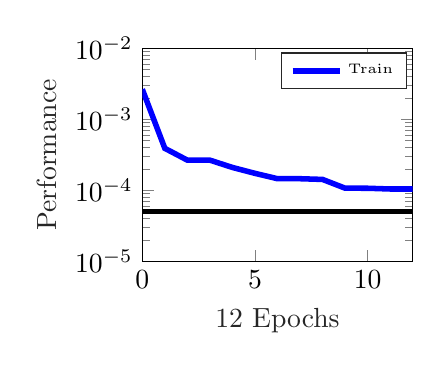
\begin{tikzpicture}

\begin{axis}[%
width=1.3521in,
height=1.066in,
at={(0.758in,0.481in)},
scale only axis,
xmin=0,
xmax=12,
xlabel style={font=\color{white!15!black}},
xlabel={12 Epochs},
ymode=log,
ymin=1e-05,
ymax=0.01,
yminorticks=true,
ylabel style={font=\color{white!15!black}},
ylabel={Performance},
axis background/.style={fill=white},
%title style={font=\bfseries},
%title={Performance is 0.000104317, Goal is 5e-05},
legend style={legend cell align=left, align=left, draw=white!15!black}
]
\addplot [color=black, line width=2.0pt, forget plot]
  table[row sep=crcr]{%
0	5e-05\\
1	5e-05\\
2	5e-05\\
3	5e-05\\
4	5e-05\\
5	5e-05\\
6	5e-05\\
7	5e-05\\
8	5e-05\\
9	5e-05\\
10	5e-05\\
11	5e-05\\
12	5e-05\\
};
\addplot [color=blue, line width=2.0pt]
  table[row sep=crcr]{%
0	0.0026443526296567\\
1	0.00038957019873408\\
2	0.000265654412531838\\
3	0.000265654412531838\\
4	0.000209674594314602\\
5	0.000173210636766609\\
6	0.00014557747800731\\
7	0.00014557747800731\\
8	0.000142221751510672\\
9	0.000107085053043968\\
10	0.000106859633411325\\
11	0.000104323198649199\\
12	0.000104316760635947\\
};
\addlegendentry{\tiny Train}

\addplot [color=mycolor1, forget plot]
  table[row sep=crcr]{%
0	0\\
};
\addplot [color=mycolor2, forget plot]
  table[row sep=crcr]{%
0	0\\
};
\end{axis}
\end{tikzpicture}% 
 \vspace{-3.5mm}
 \caption{The network’s performance according to the mean of squared errors.}
 \label{fig:MSE_state}
 \end{figure}

 \vspace{-3mm}

 \figref{fig:MSE_state} shows, that adding more neurons to the network, the performance does not increase significantly. The network has been tested with more than six neurons, however the best validation result turned out to be the best at $N = 6$ RBF neurons. The WT pressure is shown in \figref{fig:WT_ident_sigma1}



   %WT - sigma1 identification
 \begin{figure}[H]
 \centering
 %\hspace{0mm}
 %
\includegraphics[width=0.35\textwidth]{report/pictures/missingfigure}
 % This file was created by matlab2tikz.
%
%The latest updates can be retrieved from
%  http://www.mathworks.com/matlabcentral/fileexchange/22022-matlab2tikz-matlab2tikz
%where you can also make suggestions and rate matlab2tikz.
%
\definecolor{mycolor1}{rgb}{0.00000,0.44700,0.74100}%
\definecolor{mycolor2}{rgb}{0.85000,0.32500,0.09800}%
%
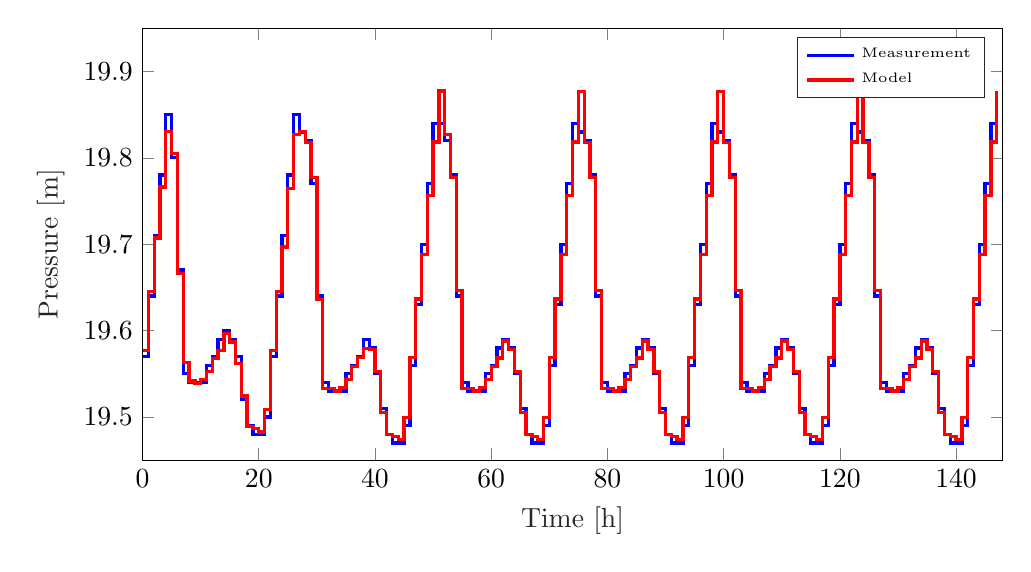
\begin{tikzpicture}

\begin{axis}[%
width=4.3in,
height=2.16in,
at={(0.548in,0.425in)},
scale only axis,
xmin=0,
xmax=148,
xlabel style={font=\color{white!15!black}},
xlabel={Time [h]},
ymin=19.45,
ymax=19.95,
ylabel style={font=\color{white!15!black}},
ylabel={Pressure  [m]},
axis background/.style={fill=white},
%title style={font=\bfseries},
%title={Inlet pressure - $\bar{p}_{\mathcal{K},1}$},
legend style={legend cell align=left, align=left, draw=white!15!black}
]
\addplot[const plot, color=blue, line width=1.2pt] table[row sep=crcr] {%
0	19.57\\
1	19.64\\
2	19.71\\
3	19.78\\
4	19.85\\
5	19.8\\
6	19.67\\
7	19.55\\
8	19.54\\
9	19.54\\
10	19.54\\
11	19.56\\
12	19.57\\
13	19.59\\
14	19.6\\
15	19.59\\
16	19.57\\
17	19.52\\
18	19.49\\
19	19.48\\
20	19.48\\
21	19.5\\
22	19.57\\
23	19.64\\
24	19.71\\
25	19.78\\
26	19.85\\
27	19.83\\
28	19.82\\
29	19.77\\
30	19.64\\
31	19.54\\
32	19.53\\
33	19.53\\
34	19.53\\
35	19.55\\
36	19.56\\
37	19.57\\
38	19.59\\
39	19.58\\
40	19.55\\
41	19.51\\
42	19.48\\
43	19.47\\
44	19.47\\
45	19.49\\
46	19.56\\
47	19.63\\
48	19.7\\
49	19.77\\
50	19.84\\
51	19.84\\
52	19.82\\
53	19.78\\
54	19.64\\
55	19.54\\
56	19.53\\
57	19.53\\
58	19.53\\
59	19.55\\
60	19.56\\
61	19.58\\
62	19.59\\
63	19.58\\
64	19.55\\
65	19.51\\
66	19.48\\
67	19.47\\
68	19.47\\
69	19.49\\
70	19.56\\
71	19.63\\
72	19.7\\
73	19.77\\
74	19.84\\
75	19.83\\
76	19.82\\
77	19.78\\
78	19.64\\
79	19.54\\
80	19.53\\
81	19.53\\
82	19.53\\
83	19.55\\
84	19.56\\
85	19.58\\
86	19.59\\
87	19.58\\
88	19.55\\
89	19.51\\
90	19.48\\
91	19.47\\
92	19.47\\
93	19.49\\
94	19.56\\
95	19.63\\
96	19.7\\
97	19.77\\
98	19.84\\
99	19.83\\
100	19.82\\
101	19.78\\
102	19.64\\
103	19.54\\
104	19.53\\
105	19.53\\
106	19.53\\
107	19.55\\
108	19.56\\
109	19.58\\
110	19.59\\
111	19.58\\
112	19.55\\
113	19.51\\
114	19.48\\
115	19.47\\
116	19.47\\
117	19.49\\
118	19.56\\
119	19.63\\
120	19.7\\
121	19.77\\
122	19.84\\
123	19.83\\
124	19.82\\
125	19.78\\
126	19.64\\
127	19.54\\
128	19.53\\
129	19.53\\
130	19.53\\
131	19.55\\
132	19.56\\
133	19.58\\
134	19.59\\
135	19.58\\
136	19.55\\
137	19.51\\
138	19.48\\
139	19.47\\
140	19.47\\
141	19.49\\
142	19.56\\
143	19.63\\
144	19.7\\
145	19.77\\
146	19.84\\
147	19.83\\
};
\addlegendentry{\tiny Measurement}

\addplot[const plot, color=red, line width=1.2pt] table[row sep=crcr] {%
0	19.5771300513152\\
1	19.6453010601766\\
2	19.7071947971859\\
3	19.7661588804339\\
4	19.8306402972678\\
5	19.8053927713787\\
6	19.6664816940618\\
7	19.5630752183405\\
8	19.5418403478368\\
9	19.5391065755239\\
10	19.5430952737288\\
11	19.5523578178391\\
12	19.5674544697418\\
13	19.577378616494\\
14	19.5967331125392\\
15	19.5869837859733\\
16	19.5620312476347\\
17	19.5243278061465\\
18	19.4892797611679\\
19	19.4865849345026\\
20	19.4827988773072\\
21	19.508587416622\\
22	19.5770405252915\\
23	19.6452662190789\\
24	19.6966025958324\\
25	19.7647423700409\\
26	19.8266851803722\\
27	19.8305956803248\\
28	19.8179910148447\\
29	19.7775568697328\\
30	19.6362565549748\\
31	19.5331117268621\\
32	19.5327410356977\\
33	19.530102226426\\
34	19.534145391671\\
35	19.5434748527053\\
36	19.5585842256376\\
37	19.5685195016145\\
38	19.5789667363354\\
39	19.5778446468138\\
40	19.5526893569823\\
41	19.5051960693716\\
42	19.4798608998333\\
43	19.477478744117\\
44	19.4737666821954\\
45	19.4997719940208\\
46	19.5685657129454\\
47	19.6367412351634\\
48	19.6880714141252\\
49	19.7562143088391\\
50	19.8181534055216\\
51	19.8771627202185\\
52	19.8271496119522\\
53	19.7775568697328\\
54	19.6463316069687\\
55	19.5331117268621\\
56	19.5327089354387\\
57	19.530102226426\\
58	19.5341087188947\\
59	19.5434748527053\\
60	19.5585842256376\\
61	19.5684798320968\\
62	19.5878499021474\\
63	19.5778446468138\\
64	19.5526893569823\\
65	19.5051960693716\\
66	19.4798608998333\\
67	19.4774466138447\\
68	19.4737666821954\\
69	19.4997719940208\\
70	19.5685657129454\\
71	19.6367412351634\\
72	19.6880714141252\\
73	19.7562143088391\\
74	19.8181534055216\\
75	19.8771294216893\\
76	19.8179910148447\\
77	19.7775568697328\\
78	19.6463316069687\\
79	19.5331117268621\\
80	19.5327089354387\\
81	19.530102226426\\
82	19.5341087188947\\
83	19.5434748527053\\
84	19.5585842256376\\
85	19.5684798320968\\
86	19.5878499021474\\
87	19.5778446468138\\
88	19.5526893569823\\
89	19.5051960693716\\
90	19.4798608998333\\
91	19.4774466138447\\
92	19.4737666821954\\
93	19.4997719940208\\
94	19.5685657129454\\
95	19.6367412351634\\
96	19.6880714141252\\
97	19.7562143088391\\
98	19.8181534055216\\
99	19.8771294216893\\
100	19.8179910148447\\
101	19.7775568697328\\
102	19.6463316069687\\
103	19.5331117268621\\
104	19.5327089354387\\
105	19.530102226426\\
106	19.5341087188947\\
107	19.5434748527053\\
108	19.5585842256376\\
109	19.5684798320968\\
110	19.5878499021474\\
111	19.5778446468138\\
112	19.5526893569823\\
113	19.5051960693716\\
114	19.4798608998333\\
115	19.4774466138447\\
116	19.4737666821954\\
117	19.4997719940208\\
118	19.5685657129454\\
119	19.6367412351634\\
120	19.6880714141252\\
121	19.7562143088391\\
122	19.8181534055216\\
123	19.8771294216893\\
124	19.8179910148447\\
125	19.7775568697328\\
126	19.6463316069687\\
127	19.5331117268621\\
128	19.5327089354387\\
129	19.530102226426\\
130	19.5341087188947\\
131	19.5434748527053\\
132	19.5585842256376\\
133	19.5684798320968\\
134	19.5878499021474\\
135	19.5778446468138\\
136	19.5526893569823\\
137	19.5051960693716\\
138	19.4798608998333\\
139	19.4774466138447\\
140	19.4737666821954\\
141	19.4997719940208\\
142	19.5685657129454\\
143	19.6367412351634\\
144	19.6880714141252\\
145	19.7562143088391\\
146	19.8181534055216\\
147	19.8771294216893\\
};
\addlegendentry{\tiny Model}

\end{axis}
\end{tikzpicture}% 
 \vspace{-2.5mm}
 \caption{Identification of the WT pressure $\hat{p}$.}
 \label{fig:WT_ident_sigma1}
 \end{figure}

 \vspace{-4mm}

The output parameter vectors $\theta_{\mathcal{K}1}$, $\theta_{\mathcal{K}2}$ and the state parameter vector $\theta_{\mathcal{S}1}$, including the output weights, linear parameters and biases are shown in \eqref{par_matrices_output_example123}.

\vspace{-2mm}

 \begin{equation}
\label{par_matrices_output_example123}
         \theta_{\mathcal{K}1} = 
          \begin{pmatrix}
           -321.27  \\
           -101.81  \\
           -391.47  \\
           -382.66  \\
           -4.48 \cdot 10^6  \\
           4.55 \cdot 10^6 \\
           9.23 \cdot 10^3 \\
           4.48 \cdot 10^6 \\
           394.62 \\
           -4.57 \cdot 10^6\\
           -0.27 \\
           37.33 \\
         \end{pmatrix}
         ,
         \hspace{5mm}
         \theta_{\mathcal{K}2} = 
          \begin{pmatrix}
           -102.36  \\
           10.88  \\
           -89.94  \\
           115.19  \\
           -3.28 \cdot 10^5  \\
           1.42 \cdot 10^5 \\
           -1.78 \cdot 10^3 \\
           3.27 \cdot 10^5 \\
           35.35 \\
           -1.39 \cdot 10^5\\
           -0.33 \\
           60.14 \\
         \end{pmatrix}
\hspace{5mm}
         \theta_{\mathcal{S}1} = 
          \begin{pmatrix}
           4.15 \cdot 10^{3} \\
            2.64 \cdot 10^{4} \\
             -5.15 \cdot 10^{4} \\
              2.51 \cdot 10^{4} \\
               0.42 \\
                -4.15 \cdot 10^{3} \\
                  3.4 \cdot 10^{-3} \\
                   -8.08 \cdot 10^{-4} \\
                   -5.8 \cdot 10^{-3} \\
                    0.16 

         \end{pmatrix}
\end{equation}

 \subsection{Validation on $\sigma_2$ total demands}
 \label{validation_sigma1}

 With the increase in total water consumption, the controls change. The new inlet flows of the two pumping stations $PU_1$, $PU_2$ and the pressure in the WT is shown in \figref{fig:WT_sigma2}.

\vspace{-2mm}

 %Inlet flow - sigma2
 \begin{figure}[H]
 \centering
 %\hspace{0mm}
 %
\includegraphics[width=0.35\textwidth]{report/pictures/missingfigure}
 % This file was created by matlab2tikz.
%
%The latest updates can be retrieved from
%  http://www.mathworks.com/matlabcentral/fileexchange/22022-matlab2tikz-matlab2tikz
%where you can also make suggestions and rate matlab2tikz.
%
\definecolor{mycolor1}{rgb}{0.00000,0.44700,0.74100}%
\definecolor{mycolor2}{rgb}{0.85000,0.32500,0.09800}%
%
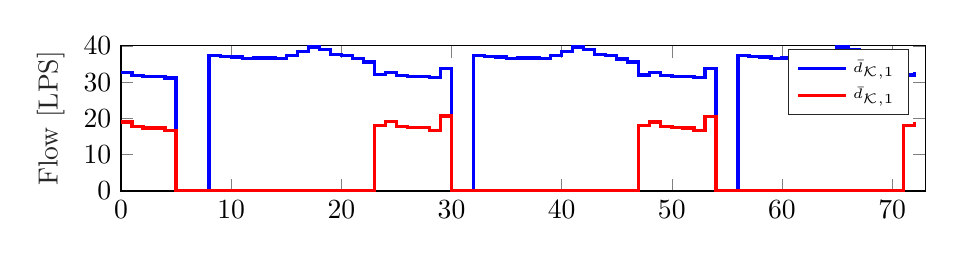
\begin{tikzpicture}

\begin{axis}[%
width=4.021in,
height=0.726in,
at={(0.852in,0.425in)},
scale only axis,
xmin=0,
xmax=73,
%xlabel style={font=\color{white!15!black}},
%xlabel={Time [h]},
ymin=0,
ymax=40,
ylabel style={font=\color{white!15!black}},
ylabel={Flow  [LPS]},
axis background/.style={fill=white},
legend style={legend cell align=left, align=left, draw=white!15!black}
]
\addplot[const plot, color=blue, line width=1.2pt] table[row sep=crcr] {%
0	32.63\\
1	31.83\\
2	31.59\\
3	31.57\\
4	31.15\\
5	0\\
6	0\\
7	0\\
8	37.37\\
9	37.06\\
10	36.91\\
11	36.59\\
12	36.68\\
13	36.63\\
14	36.56\\
15	37.41\\
16	38.47\\
17	39.69\\
18	39.02\\
19	37.62\\
20	37.38\\
21	36.42\\
22	35.53\\
23	32.01\\
24	32.67\\
25	31.87\\
26	31.63\\
27	31.61\\
28	31.19\\
29	33.81\\
30	0\\
31	0\\
32	37.35\\
33	37.03\\
34	36.88\\
35	36.56\\
36	36.65\\
37	36.61\\
38	36.53\\
39	37.38\\
40	38.44\\
41	39.66\\
42	39\\
43	37.6\\
44	37.35\\
45	36.4\\
46	35.51\\
47	31.99\\
48	32.65\\
49	31.85\\
50	31.61\\
51	31.59\\
52	31.18\\
53	33.79\\
54	0\\
55	0\\
56	37.36\\
57	37.05\\
58	36.89\\
59	36.57\\
60	36.67\\
61	36.62\\
62	36.55\\
63	37.4\\
64	38.45\\
65	39.68\\
66	39.01\\
67	37.61\\
68	37.37\\
69	36.41\\
70	35.52\\
71	32\\
72	32.66\\
};
\addlegendentry{ \tiny $\bar{d}_{\mathcal{K},1}$}

\addplot[const plot, color=red, line width=1.2pt] table[row sep=crcr] {%
0	19\\
1	17.78\\
2	17.38\\
3	17.34\\
4	16.65\\
5	0\\
6	0\\
7	0\\
8	0\\
9	0\\
10	0\\
11	0\\
12	0\\
13	0\\
14	0\\
15	0\\
16	0\\
17	0\\
18	0\\
19	0\\
20	0\\
21	0\\
22	0\\
23	18.09\\
24	19.07\\
25	17.85\\
26	17.45\\
27	17.42\\
28	16.72\\
29	20.63\\
30	0\\
31	0\\
32	0\\
33	0\\
34	0\\
35	0\\
36	0\\
37	0\\
38	0\\
39	0\\
40	0\\
41	0\\
42	0\\
43	0\\
44	0\\
45	0\\
46	0\\
47	18.06\\
48	19.04\\
49	17.82\\
50	17.42\\
51	17.38\\
52	16.69\\
53	20.59\\
54	0\\
55	0\\
56	0\\
57	0\\
58	0\\
59	0\\
60	0\\
61	0\\
62	0\\
63	0\\
64	0\\
65	0\\
66	0\\
67	0\\
68	0\\
69	0\\
70	0\\
71	18.07\\
72	19.06\\
};
\addlegendentry{\tiny $\bar{d}_{\mathcal{K},1}$}

\end{axis}
\end{tikzpicture}% 
 \vspace{-2.5mm}
 %\caption{Inlet flows of $PU_1$ and $PU_2$.}
 \label{fig:dk_sigma2}
 \end{figure}

 \vspace{-6.5mm}

   %WT - sigma2
 \begin{figure}[H]
 \centering
 \hspace{-3.5mm}
 %
\includegraphics[width=0.35\textwidth]{report/pictures/missingfigure}
 % This file was created by matlab2tikz.
%
%The latest updates can be retrieved from
%  http://www.mathworks.com/matlabcentral/fileexchange/22022-matlab2tikz-matlab2tikz
%where you can also make suggestions and rate matlab2tikz.
%
\definecolor{mycolor1}{rgb}{0.00000,0.44700,0.74100}%
%
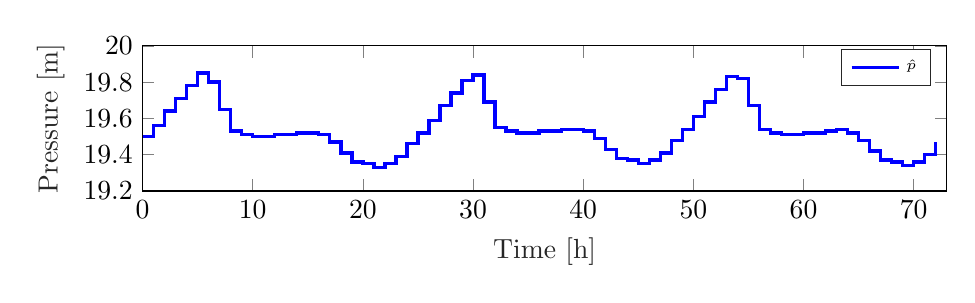
\begin{tikzpicture}

\begin{axis}[%
width=4.021in,
height=0.726in,
at={(0.833in,0.431in)},
scale only axis,
xmin=0,
xmax=73,
xlabel style={font=\color{white!15!black}},
xlabel={Time [h]},
ymin=19.2,
ymax=20,
ylabel style={font=\color{white!15!black}},
ylabel={Pressure  [m]},
axis background/.style={fill=white},
legend style={legend cell align=left, align=left, draw=white!15!black}
]
\addplot[const plot, color=blue, line width=1.2pt] table[row sep=crcr] {%
0	19.5\\
1	19.56\\
2	19.64\\
3	19.71\\
4	19.78\\
5	19.85\\
6	19.8\\
7	19.65\\
8	19.53\\
9	19.51\\
10	19.5\\
11	19.5\\
12	19.51\\
13	19.51\\
14	19.52\\
15	19.52\\
16	19.51\\
17	19.47\\
18	19.41\\
19	19.36\\
20	19.35\\
21	19.33\\
22	19.35\\
23	19.39\\
24	19.46\\
25	19.52\\
26	19.59\\
27	19.67\\
28	19.74\\
29	19.81\\
30	19.84\\
31	19.69\\
32	19.55\\
33	19.53\\
34	19.52\\
35	19.52\\
36	19.53\\
37	19.53\\
38	19.54\\
39	19.54\\
40	19.53\\
41	19.49\\
42	19.43\\
43	19.38\\
44	19.37\\
45	19.35\\
46	19.37\\
47	19.41\\
48	19.48\\
49	19.54\\
50	19.61\\
51	19.69\\
52	19.76\\
53	19.83\\
54	19.82\\
55	19.67\\
56	19.54\\
57	19.52\\
58	19.51\\
59	19.51\\
60	19.52\\
61	19.52\\
62	19.53\\
63	19.54\\
64	19.52\\
65	19.48\\
66	19.42\\
67	19.37\\
68	19.36\\
69	19.34\\
70	19.36\\
71	19.4\\
72	19.47\\
};
\addlegendentry{\tiny $\hat{p}$}

\end{axis}
\end{tikzpicture}% 
 \vspace{-2.5mm}
 \caption{Inlet flows of $PU_1$ and $PU_2$(above) and the pressure in the WT(below).}
 \label{fig:WT_sigma2}
 \end{figure}

 \vspace{-3mm}

The simulation results for $\bar{p}_{\mathcal{K}1}$ and $\bar{p}_{\mathcal{K}2}$ inlet pressures on the new validation data when $\sigma_2$ is the total demand in the network are shown in \figref{fig:pk1_sigma2}

\vspace{-2mm}

   %pk1 - pk2 - sigma2
 \begin{figure}[H]
 \centering
 %\hspace{0mm}
 %
\includegraphics[width=0.35\textwidth]{report/pictures/missingfigure}
 % This file was created by matlab2tikz.
%
%The latest updates can be retrieved from
%  http://www.mathworks.com/matlabcentral/fileexchange/22022-matlab2tikz-matlab2tikz
%where you can also make suggestions and rate matlab2tikz.
%
\definecolor{mycolor1}{rgb}{0.00000,0.44700,0.74100}%
\definecolor{mycolor2}{rgb}{0.85000,0.32500,0.09800}%
%
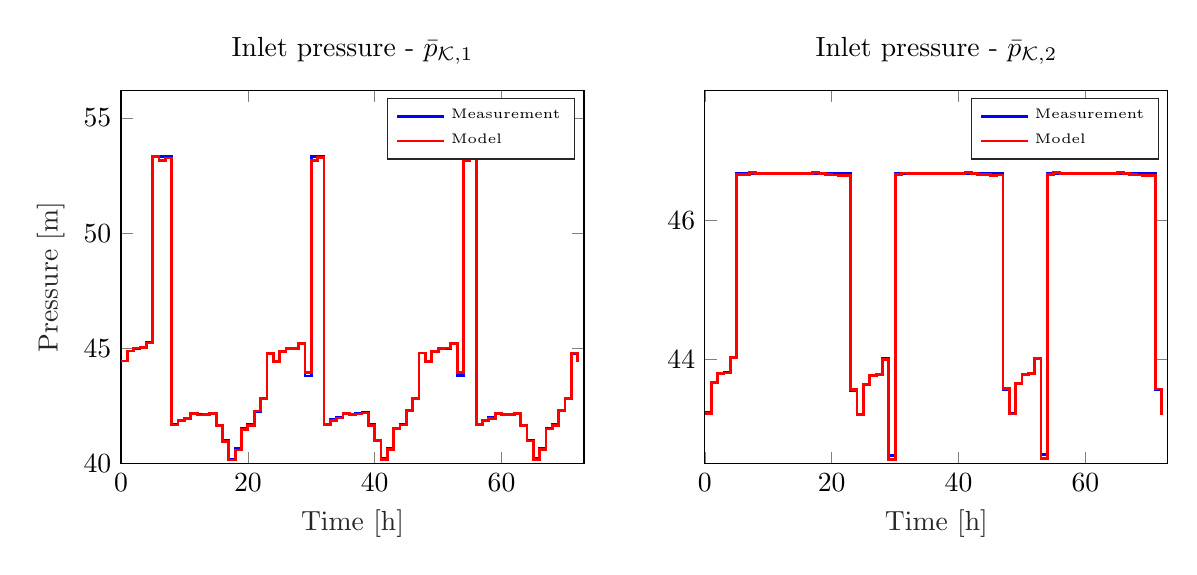
\begin{tikzpicture}

\begin{axis}[%
width=2.315in,
height=1.866in,
at={(1.071in,0.43in)},
scale only axis,
xmin=0,
xmax=73,
xlabel style={font=\color{white!15!black}},
xlabel={Time [h]},
ymin=40,
ymax=56.2,
ylabel style={font=\color{white!15!black}},
ylabel={Pressure  [m]},
axis background/.style={fill=white},
%title style={font=\bfseries},
title={Inlet pressure - $\bar{p}_{\mathcal{K},1}$},
legend style={legend cell align=left, align=left, draw=white!15!black}
]
\addplot[const plot, color=blue, line width=1pt] table[row sep=crcr] {%
0	44.4566493554\\
1	44.8864170674\\
2	45.0132672146\\
3	45.0237947234\\
4	45.243332285\\
5	53.33\\
6	53.33\\
7	53.33\\
8	41.6914281554\\
9	41.8837210376\\
10	41.9761909346\\
11	42.1722066146\\
12	42.1172497184\\
13	42.1477979954\\
14	42.1904955776\\
15	41.6664994946\\
16	40.9961725394\\
17	40.2014823026\\
18	40.6409816264\\
19	41.5351864904\\
20	41.6851984904\\
21	42.2756457224\\
22	42.8093175794\\
23	44.7906494066\\
24	44.4348809474\\
25	44.8651820354\\
26	44.9921921954\\
27	45.0027330386\\
28	45.2225506226\\
29	43.8032704226\\
30	53.33\\
31	53.33\\
32	41.703882485\\
33	41.9022450194\\
34	41.9946399104\\
35	42.1904955776\\
36	42.135583685\\
37	42.1600056386\\
38	42.2087695394\\
39	41.6851984904\\
40	41.0154015776\\
41	40.2213213896\\
42	40.653986\\
43	41.54772416\\
44	41.703882485\\
45	42.28778336\\
46	42.8211585266\\
47	44.8013169266\\
48	44.445768485\\
49	44.875802885\\
50	45.0027330386\\
51	45.0132672146\\
52	45.2277485384\\
53	43.8145379906\\
54	53.33\\
55	53.33\\
56	41.6976561536\\
57	41.889897365\\
58	41.9884919186\\
59	42.1844009234\\
60	42.1233627074\\
61	42.1539026504\\
62	42.196588565\\
63	41.67273416\\
64	41.008993565\\
65	40.2080969984\\
66	40.6474846466\\
67	41.5414561586\\
68	41.6914281554\\
69	42.2817153746\\
70	42.8152388864\\
71	44.795984\\
72	44.4403255496\\
};
\addlegendentry{\tiny Measurement}

\addplot[const plot, color=red, line width=1pt] table[row sep=crcr] {%
0	44.4511325921288\\
1	44.8916412812395\\
2	45.0178020162973\\
3	45.0275746337192\\
4	45.2360182549448\\
5	53.3195711030789\\
6	53.1480843685626\\
7	53.2648614555804\\
8	41.6751010841737\\
9	41.8648843765822\\
10	41.9594218305668\\
11	42.1661610345712\\
12	42.109775333256\\
13	42.1396376933534\\
14	42.1833392398271\\
15	41.6486613352622\\
16	40.9713099580821\\
17	40.1540949374171\\
18	40.5896841686571\\
19	41.4954412241713\\
20	41.6510661700779\\
21	42.2853297107477\\
22	42.8127137660088\\
23	44.7930457018253\\
24	44.4239274062674\\
25	44.8700361547831\\
26	44.9987752985569\\
27	45.0065180711604\\
28	45.2185671102932\\
29	43.9429093810995\\
30	53.1559050338299\\
31	53.2733789382608\\
32	41.6909613855644\\
33	41.8847778770188\\
34	41.9785640265632\\
35	42.1833392398271\\
36	42.1275336649315\\
37	42.1523162275599\\
38	42.2005078859881\\
39	41.6696922939525\\
40	40.9939333871054\\
41	40.1771114097125\\
42	40.6072946207433\\
43	41.5114226557044\\
44	41.6713811330951\\
45	42.2959582381921\\
46	42.8201144849404\\
47	44.8036415016631\\
48	44.4370513454952\\
49	44.8804379657165\\
50	45.0084486746072\\
51	45.0170650939097\\
52	45.2223612182934\\
53	43.9619487935426\\
54	53.1519962870058\\
55	53.2691217866882\\
56	41.6830319214866\\
57	41.872325846723\\
58	41.9714737800513\\
59	42.1771638664049\\
60	42.1162233951341\\
61	42.1459776887509\\
62	42.1895131529355\\
63	41.6594910237261\\
64	40.9852511294025\\
65	40.1629366072767\\
66	40.598489944879\\
67	41.5034326058335\\
68	41.6586968928822\\
69	42.2906446976419\\
70	42.8164148556315\\
71	44.7987837662134\\
72	44.4299966411363\\
};
\addlegendentry{\tiny Model}

\end{axis}

\begin{axis}[%
xshift=-1.8cm,
width=2.315in,
height=1.866in,
at={(4.699in,0.43in)},
scale only axis,
xmin=0,
xmax=73,
xlabel style={font=\color{white!15!black}},
xlabel={Time [h]},
ymin=42.5,
ymax=47.87,
%ylabel style={font=\color{white!15!black}},
%ylabel={Pressure  [m]},
axis background/.style={fill=white},
%title style={font=\bfseries},
title={Inlet pressure - $\bar{p}_{\mathcal{K},2}$},
legend style={legend cell align=left, align=left, draw=white!15!black}
]
\addplot[const plot, color=blue, line width=1pt] table[row sep=crcr] {%
0	43.231475\\
1	43.65887699\\
2	43.79283659\\
3	43.80606491\\
4	44.0294556875\\
5	46.67\\
6	46.67\\
7	46.67\\
8	46.67\\
9	46.67\\
10	46.67\\
11	46.67\\
12	46.67\\
13	46.67\\
14	46.67\\
15	46.67\\
16	46.67\\
17	46.67\\
18	46.67\\
19	46.67\\
20	46.67\\
21	46.67\\
22	46.67\\
23	43.5529618475\\
24	43.2060918275\\
25	43.6351206875\\
26	43.7696136875\\
27	43.77957779\\
28	44.00720624\\
29	42.6161895275\\
30	46.67\\
31	46.67\\
32	46.67\\
33	46.67\\
34	46.67\\
35	46.67\\
36	46.67\\
37	46.67\\
38	46.67\\
39	46.67\\
40	46.67\\
41	46.67\\
42	46.67\\
43	46.67\\
44	46.67\\
45	46.67\\
46	46.67\\
47	43.56329171\\
48	43.21698176\\
49	43.64531339\\
50	43.77957779\\
51	43.79283659\\
52	44.0167531475\\
53	42.6318943475\\
54	46.67\\
55	46.67\\
56	46.67\\
57	46.67\\
58	46.67\\
59	46.67\\
60	46.67\\
61	46.67\\
62	46.67\\
63	46.67\\
64	46.67\\
65	46.67\\
66	46.67\\
67	46.67\\
68	46.67\\
69	46.67\\
70	46.67\\
71	43.5598503275\\
72	43.20972371\\
};
\addlegendentry{\tiny Measurement}

\addplot[const plot, color=red, line width=1pt] table[row sep=crcr] {%
0	43.2247474200768\\
1	43.6622949844258\\
2	43.7941491199819\\
3	43.8028423058792\\
4	44.0237893434762\\
5	46.6625420063299\\
6	46.6654049636243\\
7	46.6859167697385\\
8	46.6764023014698\\
9	46.6747414383907\\
10	46.6725618902484\\
11	46.6690391105868\\
12	46.6706710183397\\
13	46.6712454682028\\
14	46.6724215802412\\
15	46.6752933158884\\
16	46.6762617292015\\
17	46.6833286430899\\
18	46.6748886969099\\
19	46.6569718958108\\
20	46.6532637751736\\
21	46.6440107500063\\
22	46.6496452125505\\
23	43.5675204766443\\
24	43.2021628313232\\
25	43.6408350507724\\
26	43.7720488265506\\
27	43.7797475171697\\
28	44.0032869470034\\
29	42.5639392090403\\
30	46.6598316981872\\
31	46.6813911143883\\
32	46.6783279160264\\
33	46.6776245134247\\
34	46.6756273534872\\
35	46.6724215802412\\
36	46.673979307438\\
37	46.6739248312374\\
38	46.6758015630024\\
39	46.6778067667022\\
40	46.6777933258131\\
41	46.683896077005\\
42	46.6755043093641\\
43	46.6588801892664\\
44	46.6560644766322\\
45	46.646884911381\\
46	46.6525289851159\\
47	43.5773190088176\\
48	43.2124349371839\\
49	43.6505995672908\\
50	43.7816604488897\\
51	43.7912982104728\\
52	44.0116770353613\\
53	42.5769087338687\\
54	46.6626183540506\\
55	46.68365396117\\
56	46.6773652186514\\
57	46.6758663465759\\
58	46.6744168685299\\
59	46.6710614992379\\
60	46.671996577267\\
61	46.6725852786355\\
62	46.673781400707\\
63	46.6765778349057\\
64	46.6773102751055\\
65	46.683355194949\\
66	46.6751965750525\\
67	46.6579261443147\\
68	46.6543470721281\\
69	46.6454479596964\\
70	46.651087241442\\
71	43.5733912397529\\
72	43.2062767543266\\
};
\addlegendentry{\tiny Model}

\end{axis}
\end{tikzpicture}% 
 \vspace{-2.5mm}
 \caption{Simulation of $\bar{p}_{\mathcal{K}1}$ and $\bar{p}_{\mathcal{K}2}$ pressures on validation data.}
 \label{fig:pk1_sigma2}
 \end{figure}

 \vspace{-4mm}

 The simulation results for $\hat{p}$ WT pressure on the new validation data when $\sigma_2$ is the total demand in the network are shown in \figref{fig:WT_ident_sigma2}

   %WT - sigma2 identification
 \begin{figure}[H]
 \centering
 %\hspace{0mm}
 %
\includegraphics[width=0.35\textwidth]{report/pictures/missingfigure}
 % This file was created by matlab2tikz.
%
%The latest updates can be retrieved from
%  http://www.mathworks.com/matlabcentral/fileexchange/22022-matlab2tikz-matlab2tikz
%where you can also make suggestions and rate matlab2tikz.
%
\definecolor{mycolor1}{rgb}{0.00000,0.44700,0.74100}%
\definecolor{mycolor2}{rgb}{0.85000,0.32500,0.09800}%
%
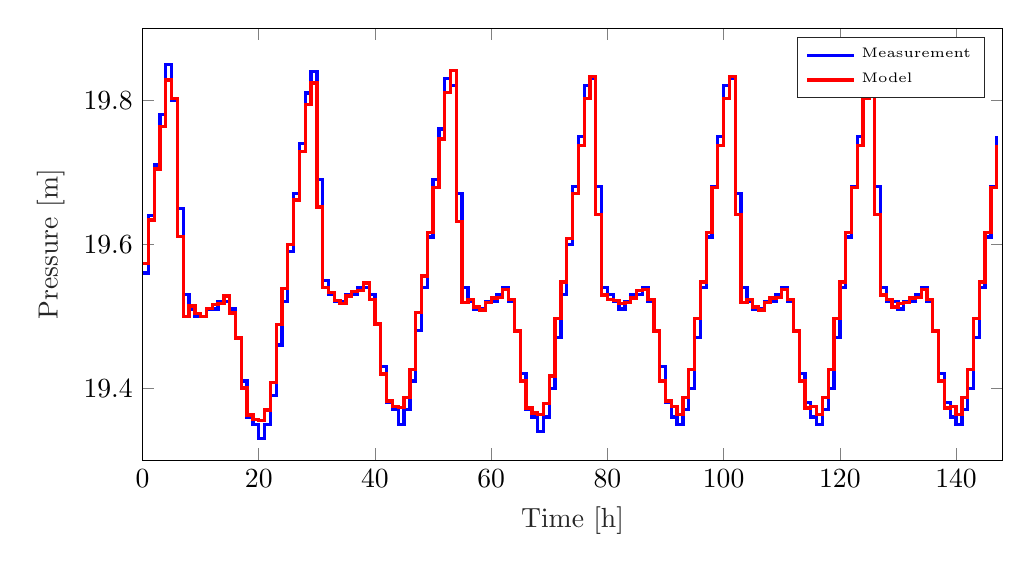
\begin{tikzpicture}

\begin{axis}[%
width=4.3in,
height=2.16in,
at={(0.712in,0.433in)},
scale only axis,
xmin=0,
xmax=148,
xlabel style={font=\color{white!15!black}},
xlabel={Time [h]},
ymin=19.3,
ymax=19.9,
ylabel style={font=\color{white!15!black}},
ylabel={Pressure  [m]},
axis background/.style={fill=white},
legend style={legend cell align=left, align=left, draw=white!15!black}
]
\addplot[const plot, color=blue, line width=1.2pt] table[row sep=crcr] {%
0	19.56\\
1	19.64\\
2	19.71\\
3	19.78\\
4	19.85\\
5	19.8\\
6	19.65\\
7	19.53\\
8	19.51\\
9	19.5\\
10	19.5\\
11	19.51\\
12	19.51\\
13	19.52\\
14	19.52\\
15	19.51\\
16	19.47\\
17	19.41\\
18	19.36\\
19	19.35\\
20	19.33\\
21	19.35\\
22	19.39\\
23	19.46\\
24	19.52\\
25	19.59\\
26	19.67\\
27	19.74\\
28	19.81\\
29	19.84\\
30	19.69\\
31	19.55\\
32	19.53\\
33	19.52\\
34	19.52\\
35	19.53\\
36	19.53\\
37	19.54\\
38	19.54\\
39	19.53\\
40	19.49\\
41	19.43\\
42	19.38\\
43	19.37\\
44	19.35\\
45	19.37\\
46	19.41\\
47	19.48\\
48	19.54\\
49	19.61\\
50	19.69\\
51	19.76\\
52	19.83\\
53	19.82\\
54	19.67\\
55	19.54\\
56	19.52\\
57	19.51\\
58	19.51\\
59	19.52\\
60	19.52\\
61	19.53\\
62	19.54\\
63	19.52\\
64	19.48\\
65	19.42\\
66	19.37\\
67	19.36\\
68	19.34\\
69	19.36\\
70	19.4\\
71	19.47\\
72	19.53\\
73	19.6\\
74	19.68\\
75	19.75\\
76	19.82\\
77	19.83\\
78	19.68\\
79	19.54\\
80	19.53\\
81	19.52\\
82	19.51\\
83	19.52\\
84	19.53\\
85	19.53\\
86	19.54\\
87	19.52\\
88	19.48\\
89	19.43\\
90	19.38\\
91	19.36\\
92	19.35\\
93	19.37\\
94	19.4\\
95	19.47\\
96	19.54\\
97	19.61\\
98	19.68\\
99	19.75\\
100	19.82\\
101	19.83\\
102	19.67\\
103	19.54\\
104	19.52\\
105	19.51\\
106	19.51\\
107	19.52\\
108	19.52\\
109	19.53\\
110	19.54\\
111	19.52\\
112	19.48\\
113	19.42\\
114	19.38\\
115	19.36\\
116	19.35\\
117	19.37\\
118	19.4\\
119	19.47\\
120	19.54\\
121	19.61\\
122	19.68\\
123	19.75\\
124	19.82\\
125	19.83\\
126	19.68\\
127	19.54\\
128	19.52\\
129	19.52\\
130	19.51\\
131	19.52\\
132	19.52\\
133	19.53\\
134	19.54\\
135	19.52\\
136	19.48\\
137	19.42\\
138	19.38\\
139	19.36\\
140	19.35\\
141	19.37\\
142	19.4\\
143	19.47\\
144	19.54\\
145	19.61\\
146	19.68\\
147	19.75\\
};
\addlegendentry{\tiny Measurement}

\addplot[const plot, color=red, line width=1.2pt] table[row sep=crcr] {%
0	19.5731004307818\\
1	19.6334823450766\\
2	19.7042706539293\\
3	19.7631331076782\\
4	19.8280615045308\\
5	19.8026816773578\\
6	19.6109717871339\\
7	19.4992223393441\\
8	19.514215573284\\
9	19.503844941615\\
10	19.4994808028787\\
11	19.510275136352\\
12	19.5162286075918\\
13	19.5173764843182\\
14	19.5281297164143\\
15	19.5042974571438\\
16	19.4699354774073\\
17	19.4004408799653\\
18	19.3628042168276\\
19	19.3561537531271\\
20	19.3547441287097\\
21	19.3695842298458\\
22	19.4081927369785\\
23	19.4885390179194\\
24	19.5389121994749\\
25	19.5993500010259\\
26	19.6614820757639\\
27	19.7290228455985\\
28	19.7938924818684\\
29	19.8238761077105\\
30	19.6516916361923\\
31	19.5396735744466\\
32	19.532735541671\\
33	19.5221082825458\\
34	19.5176095548773\\
35	19.5281297164143\\
36	19.5341545839995\\
37	19.535310698798\\
38	19.5459846173317\\
39	19.5228064881294\\
40	19.4889707826417\\
41	19.4198613373576\\
42	19.3820223954751\\
43	19.3746885770914\\
44	19.3730734537577\\
45	19.3872930838203\\
46	19.4257147849249\\
47	19.5056178525157\\
48	19.5560237918948\\
49	19.616433367416\\
50	19.6785687470395\\
51	19.7460775055856\\
52	19.8110457227283\\
53	19.8412265542411\\
54	19.6313317243769\\
55	19.519447968294\\
56	19.5234755222691\\
57	19.5129923452\\
58	19.5085283723072\\
59	19.5191834024206\\
60	19.5252099182431\\
61	19.5263435669799\\
62	19.5370760779854\\
63	19.5228632359349\\
64	19.4794415200809\\
65	19.4101612944182\\
66	19.3724132632141\\
67	19.3654211321674\\
68	19.3639243956489\\
69	19.3784386400328\\
70	19.4169537456322\\
71	19.4970605096591\\
72	19.5474857123688\\
73	19.6078740142559\\
74	19.6700079925373\\
75	19.7375500585837\\
76	19.8024594259987\\
77	19.8325512616578\\
78	19.6415116834761\\
79	19.5295607742207\\
80	19.5234469441412\\
81	19.522139811533\\
82	19.5176095548773\\
83	19.5191834024206\\
84	19.5251731931744\\
85	19.535310698798\\
86	19.5370381789192\\
87	19.5228348560768\\
88	19.4794415200809\\
89	19.4101407827079\\
90	19.3820223954751\\
91	19.3746885770914\\
92	19.3638930920055\\
93	19.3872930838203\\
94	19.4257147849249\\
95	19.4970060135805\\
96	19.5473965303233\\
97	19.6165223110138\\
98	19.6786033692618\\
99	19.7375156766427\\
100	19.8024260356906\\
101	19.8325200398325\\
102	19.6415116834761\\
103	19.519447968294\\
104	19.5234755222691\\
105	19.5129607799495\\
106	19.5085283723072\\
107	19.5191834024206\\
108	19.5251731931744\\
109	19.5263435669799\\
110	19.5370381789192\\
111	19.5228348560768\\
112	19.4794415200809\\
113	19.4101407827079\\
114	19.3724132632141\\
115	19.3747176397909\\
116	19.3638930920055\\
117	19.3873349329529\\
118	19.4257608255403\\
119	19.4970605096591\\
120	19.547450152763\\
121	19.6165223110138\\
122	19.6786568176752\\
123	19.7375156766427\\
124	19.8024260356906\\
125	19.8325512616578\\
126	19.6415116834761\\
127	19.5295607742207\\
128	19.5234755222691\\
129	19.5129607799495\\
130	19.5176430426832\\
131	19.5191834024206\\
132	19.5251731931744\\
133	19.526306368894\\
134	19.5370381789192\\
135	19.5228348560768\\
136	19.4794415200809\\
137	19.4101407827079\\
138	19.372390996008\\
139	19.3747176397909\\
140	19.3638930920055\\
141	19.3873349329529\\
142	19.4257147849249\\
143	19.4970060135805\\
144	19.5473965303233\\
145	19.6165223110138\\
146	19.6786033692618\\
147	19.7375156766427\\
};
\addlegendentry{\tiny Model}

\end{axis}
\end{tikzpicture}% 
 \vspace{-2.5mm}
 \caption{Identification of the WT pressure $\hat{p}$.}
 \label{fig:WT_ident_sigma2}
 \end{figure}

 \vspace{-4mm}


\subsection{Validation on $\sigma_3$ total demands}
 \label{validation_sigma2}


\vspace{-2mm}

 %Inlet flow - sigma3
 \begin{figure}[H]
 \centering
 %\hspace{0mm}
 %
\includegraphics[width=0.35\textwidth]{report/pictures/missingfigure}
 % This file was created by matlab2tikz.
%
%The latest updates can be retrieved from
%  http://www.mathworks.com/matlabcentral/fileexchange/22022-matlab2tikz-matlab2tikz
%where you can also make suggestions and rate matlab2tikz.
%
\definecolor{mycolor1}{rgb}{0.00000,0.44700,0.74100}%
\definecolor{mycolor2}{rgb}{0.85000,0.32500,0.09800}%
%
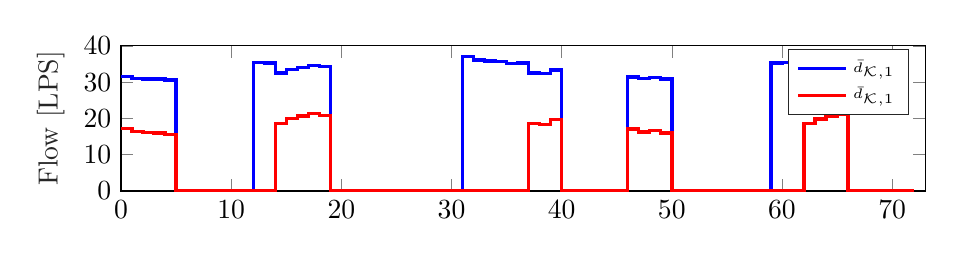
\begin{tikzpicture}

\begin{axis}[%
width=4.021in,
height=0.726in,
at={(0.86in,0.426in)},
scale only axis,
xmin=0,
xmax=73,
%xlabel style={font=\color{white!15!black}},
%xlabel={Time [h]},
ymin=0,
ymax=40,
ylabel style={font=\color{white!15!black}},
ylabel={Flow  [LPS]},
axis background/.style={fill=white},
legend style={legend cell align=left, align=left, draw=white!15!black}
]
\addplot[const plot, color=blue, line width=1.2pt] table[row sep=crcr] {%
0	31.51\\
1	31.04\\
2	30.87\\
3	30.83\\
4	30.57\\
5	0\\
6	0\\
7	0\\
8	0\\
9	0\\
10	0\\
11	0\\
12	35.39\\
13	35.3\\
14	32.51\\
15	33.49\\
16	34.1\\
17	34.56\\
18	34.21\\
19	0\\
20	0\\
21	0\\
22	0\\
23	0\\
24	0\\
25	0\\
26	0\\
27	0\\
28	0\\
29	0\\
30	0\\
31	37.02\\
32	36.07\\
33	35.81\\
34	35.63\\
35	35.22\\
36	35.28\\
37	32.54\\
38	32.39\\
39	33.37\\
40	0\\
41	0\\
42	0\\
43	0\\
44	0\\
45	0\\
46	31.45\\
47	30.98\\
48	31.3\\
49	30.83\\
50	0\\
51	0\\
52	0\\
53	0\\
54	0\\
55	0\\
56	0\\
57	0\\
58	0\\
59	35.29\\
60	35.36\\
61	35.27\\
62	32.48\\
63	33.46\\
64	34.08\\
65	34.54\\
66	0\\
67	0\\
68	0\\
69	0\\
70	0\\
71	0\\
72	0\\
};
\addlegendentry{\tiny $\bar{d}_{\mathcal{K},1}$}

\addplot[const plot, color=red, line width=1.2pt] table[row sep=crcr] {%
0	17.15\\
1	16.4\\
2	16.11\\
3	16.01\\
4	15.57\\
5	0\\
6	0\\
7	0\\
8	0\\
9	0\\
10	0\\
11	0\\
12	0\\
13	0\\
14	18.55\\
15	19.89\\
16	20.69\\
17	21.27\\
18	20.81\\
19	0\\
20	0\\
21	0\\
22	0\\
23	0\\
24	0\\
25	0\\
26	0\\
27	0\\
28	0\\
29	0\\
30	0\\
31	0\\
32	0\\
33	0\\
34	0\\
35	0\\
36	0\\
37	18.59\\
38	18.36\\
39	19.7\\
40	0\\
41	0\\
42	0\\
43	0\\
44	0\\
45	0\\
46	17.04\\
47	16.28\\
48	16.76\\
49	16.01\\
50	0\\
51	0\\
52	0\\
53	0\\
54	0\\
55	0\\
56	0\\
57	0\\
58	0\\
59	0\\
60	0\\
61	0\\
62	18.51\\
63	19.85\\
64	20.65\\
65	21.23\\
66	0\\
67	0\\
68	0\\
69	0\\
70	0\\
71	0\\
72	0\\
};
\addlegendentry{\tiny $\bar{d}_{\mathcal{K},1}$}

\end{axis}
\end{tikzpicture}% 
 \vspace{-2.5mm}
 %\caption{Inlet flows of $PU_1$ and $PU_2$.}
 \label{fig:dk_sigma3}
 \end{figure}

 \vspace{-6.5mm}

   %WT - sigma2
 \begin{figure}[H]
 \centering
 \hspace{-3.5mm}
 %
\includegraphics[width=0.35\textwidth]{report/pictures/missingfigure}
 % This file was created by matlab2tikz.
%
%The latest updates can be retrieved from
%  http://www.mathworks.com/matlabcentral/fileexchange/22022-matlab2tikz-matlab2tikz
%where you can also make suggestions and rate matlab2tikz.
%
\definecolor{mycolor1}{rgb}{0.00000,0.44700,0.74100}%
%
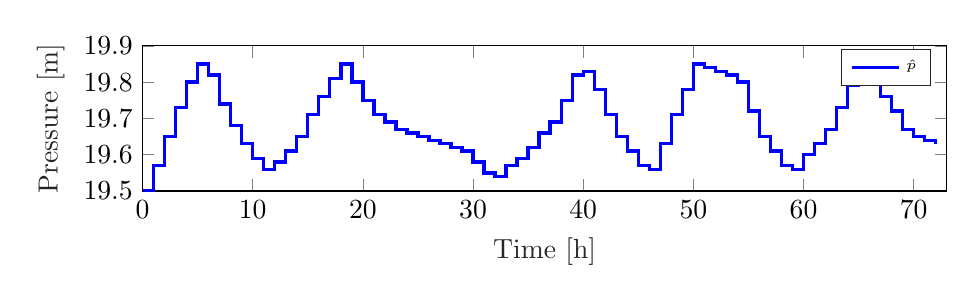
\begin{tikzpicture}

\begin{axis}[%
width=4.021in,
height=0.726in,
at={(0.765in,0.433in)},
scale only axis,
xmin=0,
xmax=73,
xlabel style={font=\color{white!15!black}},
xlabel={Time [h]},
ymin=19.5,
ymax=19.9,
ylabel style={font=\color{white!15!black}},
ylabel={Pressure  [m]},
axis background/.style={fill=white},
legend style={legend cell align=left, align=left, draw=white!15!black}
]
\addplot[const plot, color=blue, line width=1.2pt] table[row sep=crcr] {%
0	19.5\\
1	19.57\\
2	19.65\\
3	19.73\\
4	19.8\\
5	19.85\\
6	19.82\\
7	19.74\\
8	19.68\\
9	19.63\\
10	19.59\\
11	19.56\\
12	19.58\\
13	19.61\\
14	19.65\\
15	19.71\\
16	19.76\\
17	19.81\\
18	19.85\\
19	19.8\\
20	19.75\\
21	19.71\\
22	19.69\\
23	19.67\\
24	19.66\\
25	19.65\\
26	19.64\\
27	19.63\\
28	19.62\\
29	19.61\\
30	19.58\\
31	19.55\\
32	19.54\\
33	19.57\\
34	19.59\\
35	19.62\\
36	19.66\\
37	19.69\\
38	19.75\\
39	19.82\\
40	19.83\\
41	19.78\\
42	19.71\\
43	19.65\\
44	19.61\\
45	19.57\\
46	19.56\\
47	19.63\\
48	19.71\\
49	19.78\\
50	19.85\\
51	19.84\\
52	19.83\\
53	19.82\\
54	19.8\\
55	19.72\\
56	19.65\\
57	19.61\\
58	19.57\\
59	19.56\\
60	19.6\\
61	19.63\\
62	19.67\\
63	19.73\\
64	19.79\\
65	19.83\\
66	19.82\\
67	19.76\\
68	19.72\\
69	19.67\\
70	19.65\\
71	19.64\\
72	19.63\\
};
\addlegendentry{\tiny $\hat{p}$}

\end{axis}
\end{tikzpicture}% 
 \vspace{-2.5mm}
 \caption{Inlet flows of $PU_1$ and $PU_2$(above) and the pressure in the WT(below).}
 \label{fig:WT_sigma3}
 \end{figure}

 \vspace{-3mm}


\chapter{Example network description}
\label{physical_properties_example1}

\emph{In this part of the appendix, the corresponding physical parameters, control properties and consumption properties of the Multi-inlet, Single-WT example network are listed.}

%Work in progress
\begin{figure}[H]
\centering

\includegraphics[width=0.4\textwidth]{report/pictures/missingfigure}
\end{figure}




